\section{La mera optimización ganadora}
En esta sección se expandió sobre las técnicas ganadoras. Se intentó ver a HPL desde todos los ángulos posibles, intentando aumentar FLOPs con todas las herramientas que se tuvo.

\subsection{Archivo de configuración}

\begin{itemize}
	\item \textbf{N}: Este es parámetro que más impacta el resultado. Define el tamaño de la matriz. El objetivo debe ser siempre elegir el valor más grande que quepa en RAM para maximizar la proporción de computación efectiva \cite{studentasc}, sin causar que el sistema haga swapping. Hay que tener en cuenta que el sistema operativo ocupa espacio en memoria, por lo que la matriz no debe ocupar el 100\% de la RAM. El porcentaje óptimo de memoria a ocupar está alrededor del 80\% \cite{studentasc}.
	Existe una fórmula para hallar el N que representa el tamaño de la memoria:
    \begin{equation*}
        \sqrt{(TotalMem \times (1024^3) \times Nodos) /8}
    \end{equation*}
    
    Donde \textit{TotalMem} es el tamaño de la memoria en GB y \textit{Nodos} es el número de nodos. También se pued multiplicar por el factor que representa el porcentaje de memoria que se quisiera usar, por ejemplo, para el 90\% se tiene:
    
    \begin{equation*}
        \sqrt{(TotalMem \times (1024^3) \times Nodos) /8} \times 0.90
    \end{equation*}
    
    En nuestros nodos, había alrededor de 61.3 GiB libres en cada uno. No se puede utilizar completamente esta cifra, pues los buffers de memoria y MPI necesitan espacio.
	
	\item \textbf{NB}: Define el tamaño del bloque para la distribución de datos. En general son menores a 256 y los mejores valores suelen ser múltiplos de 32 \cite{netlib-hpl-faq}. Además, se consideró que lo mejor es que N fuera divisible entre NB, para hacer un uso más eficiente de la memoria. Para este trabajo se estableció un valor de 256, ya que en varias fuentes se evidenció que era el mejor para nuestro procesador.
	
	\item \textbf{P$\times$Q}: El producto de \textbf{P} y \textbf{Q} es la cantidad de procesos que HPL va a utilizar. \textbf{Q} debe ser un poco mayor de \textbf{P}.
	
	Para la versión de Intel HPL, la cantidad óptima de procesos es la cantidad de sockets que se tienen.
	
	\item Panel Factorization: Hay tres opciones para factorizar el panel: left, crout, y right. Depende de la máquina de cual opción es la mejor. Para nuestros nodos la opción mas rápida fue right. Esto se puede modificar cambiando los PFACs.
    \item Recursion Factorization: Hay tres opciones para factorizar la recursión: left, crout, y right. Depende de la maquina cual es la mejor opción. Para nuestros nodos la opción más rápida fue right. Esto se puede modificar cambiando los RFACs.
    \item Panel Broadcast: Las mejores configuraciones de panel broadcast son increasing ring modified 1 y 2. Esto es porque mandan la información mucho más rápido al segundo nodo haciendo que toda la comunicación se mueva mas rápido.
    \item Look ahead: Este parámetro hace que el programa mande información al siguiente panel. Esto lo cambias modificando el parametro de depth. Puede mejorar la velocidad de procesamiento pero hay que tener cuidado porque toma mucha memoria.
    \item Update: Hay dos formas de update binary-exchange y long. Long normalmente es mejor para problemas mas grandes. Esto lo puedes cambiar cambiando el número del SWAP. Además se puso el threshold swapping en 128.
	
\end{itemize}

\subsection{Flags de compilación}
Para optimizar la compilación de HPL de Intel se usaron varias flags de compilación.

\begin{itemize}
    \item -Ofast: Es una flag que incluye varias otras flags que son -O3, -no-prec-div, y -fp-model fast=2. -O3 optimiza el programa para algoritmos que tienen complejidad $ O(n^3)$. -no-prec-div le quita precisión a las operaciones de punto flotante. -fp-model fast=2 hace que el programa corra lo mas rápido posible.
    \item -xHost: Le dice al compilador que produzca instrucciones para el host.\cite{intel-xhost}
    \item -ansi-alias: Pone las reglas de ANSI en effecto.
    \item -fdefer-pop: Quita las funciones justo cuando retornan sus valores.
    \item -foptimize-sibling-calls: Optimiza las funciones de recursión de cola.
    \item -mbranches-within-32B-boundaries: Fusiona las ramas con limites 32-byte para mejorar rendimiento.
    \item -ip: Determina si están habilitadas las optimizaciones entre procedimientos adicionales para la compilación de un solo archivo.
    \item -qoverride-limits: Deja sobreponer sobre unos limites del compilador. Previene uso excesivo de la memoria.
    \item -use-intel-optimized-headers: Determina si el directorio de encabezados de rendimiento se agrega a la lista de búsqueda de ruta.
    \item -pcn 64: Pone la precisión de los número flotante en doble.
    \item -mkl=parallel: Importa la librería de paralelo del Math Kernel Library.
    \item -Wall: Pone diagnósticos de warning y error.
    \item -fPIC: Determina si el compilador código es de posición independiente.
\end{itemize}

\subsection{Variables de ambiente de MPI}

Se utilizó el protocolo de datagramas de usuario (UDP) para realizar el intercambio de mensajes de MPI debido a que es una alternativa mas escalable que consume menos memoria, este se activó utilizando los comand:\cite{hpl_params_intel}
\begin{itemize}
    \item export I\_MPI\_FABRICS=shm:dapl
    \item export I\_MPI\_DAPL\_UD=1
\end{itemize}
Para que se haga la transferencia utilizando RDMA se utilizó el comando:
\begin{itemize}
    \item export I\_MPI\_DAPL\_UD\_PROVIDER=ofa-v2-ib0
\end{itemize}
Se deshabilitó la opción de utilizar una fábrica de comunicación distinta de DAPL en caso de no poder inicializarla mediante el comando:
\begin{itemize}
    \item export I\_MPI\_FALLBACK=0
\end{itemize}
Se quería ver la cantidad de datos enviada por cada proceso, así como información de tiempos en las funciones de MPI, esto se realizo usando:
\begin{itemize}
    \item export I\_MPI\_STATS=1-20
\end{itemize}
Para guardar esa información se eligió una carpeta usando
\begin{itemize}
    \item export I\_MPI\_STATS\_FILE=$<$path de la carpeta$>$
\end{itemize}
Se estableció el número de procesos por nodo en 4 utilizando:
\begin{itemize}
    \item export I\_MPI\_PERHOST=4
\end{itemize}
Para evitar que el agendador de MPI establezca el número de procesos por nodo físico y que sea el que se estableció se debe deshabilitar el asignador de procesos usando:
\begin{itemize}
    \item export I\_MPI\_JOB\_RESPECT\_PROCESS\_\\PLACEMENT=0
\end{itemize}
También se realizaron optimizaciones sobre los algoritmos utilizados para realizar ciertas operaciones de MPI que se utilizan en HPL. Estas fueron:
\begin{itemize}
    \item \textbf{Allgather y allgatherv:}\\
    Para realizar esta operación el algoritmo ring resulta ser mas eficiente para mensajes de más de 512K y cuando se transmiten mensajes de menor longitud el algoritmo recursive doubling es mejor. Para establecer estos algoritmos se utilizan los comandos:\\
    \begin{itemize}
        \item export I\_MPI\_ADJUST\_ALLGATHER=”1:0-524288;3”
        \item export I\_MPI\_ADJUST\_ALLGATHERV=”1: 0-524288;3”
    \end{itemize}
    \item \textbf{Reduce:}\\
    Para operaciones con datos de menos de 2Kb el algoritmo binomial resulta más eficiente mientras que para operaciones con mas tamaño de datos es más eficiente el algoritmo de Rabenseifner, esto se estableció con el comando:
    \begin{itemize}
        \item export I\_MPI\_ADJUST\_REDUCE=”2:0-2048;5”
    \end{itemize}
    \item \textbf{Allreduce:}\\
    El caso de la operación allreduce es similar al de reduce, sin embargo el algoritmo más eficiente con menos de 2Kb es el algoritmo recursive doubling, se estableció con:
    \begin{itemize}
        \item export I\_MPI\_ADJUST\_ALLREDUCE=”1:0-2048;2”
    \end{itemize}
    \item \textbf{Broadcast:}\\
    En el caso del broadcast el algoritmo que nos da un mejor performance con mensajes de menos de 12 Kb resulta ser el binomial, se estableció con:
    \begin{itemize}
        \item export I\_MPI\_ADJUST\_BCAST=”1:1-12288”
    \end{itemize}
\end{itemize}

\section{High Performance Linpack Benchmark}

Usamos el benchmark HPL incluido en la biblioteca OneAPI; este punto de referencia está disponible en
\textit{oneapi/mkl/2021.4.0/benchmarks/mp\_linpack/}.
El directorio mencionado anteriormente incluye: (1)
\textit{xhpl\_intel64\_dynamic}: un binario de referencia HPL listo para usar; (2) \textit{runme\_intel64\_dynamic}: un script de shell donde se establecen las variables de entorno MPI, aquí el binario de referencia HPL se llama con la biblioteca MPI; (3) \textit{HPL.dat}: el archivo de parámetros de HPL.

\section{Resultado sorprendente}

Después de todo este trabajo de optimización se pudo obtener un resultado 953.95 GFLOPs, equivalente a una eficiencia de 95.54\%.\\

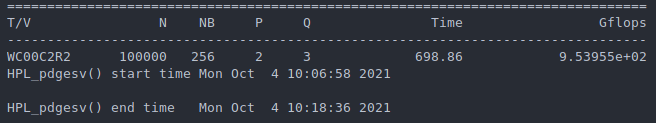
\includegraphics[width=8cm]{GFLOPS953.png}


\section{Quantum Exact Simulation Toolkit (QuEST)}

QuEST es un simulador de circuito cuántico que representa el estado del sistema cuántico utilizando vectores y matrices de densidad.

La descripción del estado de un sistema cuántico de $n$ qubits requiere $2^{n}$ números complejos. Por lo tanto, se cree que la complejidad subyacente en la simulación de computadoras cuánticas utilizando máquinas clásicas es exponencial con respecto al número de qubits.\cite{jones2019quest}.

\subsection {Informe de optimizaciones del compilador}

Para conocer las optimizaciones automáticas realizadas por el compilador en el código fuente de QuEST, se colocó la marca de informe de optimización del rendimiento, \textit{-qopt-report = 5}, además de las otras marcas del compilador Intel C.
Para esta utilidad de informe se consideró el nivel de informe más alto (cinco).
Esta utilidad de informes genera varios archivos \textit{.optrpt}, uno por archivo \textit{.cpp} en QuEST.\cite{meta2}

\subsection{Optimizaciones de rendimiento}

Ejecutamos los problemas ronda preliminar random.c, GHZ QFT y el problema 4 usando solo procesos MPI Distribuido. El rendimiento entregado en la configuración distribuida se utilizó como línea base para el cálculo de la aceleración y la validación de cada mejora de rendimiento.
La primera mejora de rendimiento aplicada fue la adición de Multi-threading, que se aplicó agregando soporte para multi-threading en el archivo QuEST makefile de cada problema.

\subsection{Variables de ambiente de MPI y SLURM}

\begin{itemize}
  \item export OMP\_NUM\_THREADS=16
  \item export I\_MPI\_CC=icx
  \item export I\_MPI\_PMI\_LIBRARY=/opt/slurm/20.11.5/lib/libpmi2.so
  \item export SLURM\_CPU\_BIND="quiet,boards"
  \item export SLURM\_PMI\_KVS\_NO\_DUP\_KEYS=1
  \item export SLURM\_MPI\_TYPE=pmi2
  \item export CC=icx
  \item export CXX=icpx
  \item export FC=ifort
  \item export F90=ifort
  \item export F77=ifort
  \item export MPIF90=mpiifort
  \item export LD=ld
  \item export AR=ar
  \item export UCX\_NET\_DEVICES=mlx4\_0:1
\end{itemize}
